\documentclass[10pt,a4paper]{article}
%]{report}

\usepackage[a4paper, top=2cm, bottom=2.5cm, left=3cm, right=3cm]{geometry}
%\usepackage[
%    vmarginratio=2:2.5, %Verh�ltnis der oben/unten Seitenr�nder zur automatischen Berechnung
%    paper=a4paper,
%    lmargin=3cm, % mittlerer Rand
%    rmargin=3cm, % �u�erer Rand
%    marginparwidth=2.3cm, % Breite des Marginpars
%    includehead, % Kopfzeile in Berechnung einbeziehen
%    includemp % Marginpar in die Berechnung mit einbeziehen
%]{geometry}
%\setlength\marginparwidth{2.3cm} %Die wird sp�ter zum Rechnen gebraucht, wird aber durch die Angabe im geometry package nicht automatisch richtig gesetzt.


%============================================================
% Pakete
%============================================================

\usepackage[english, ngerman]{babel}    % mehrsprachiger Textsatz
\usepackage[utf8]{inputenc}       % Eingabekodierung Parameter latin1 darf ge�ndert werden
\usepackage[T1]{fontenc}                % Schriftenkodierung
\usepackage{graphicx}                       % zum Einbinden von Grafiken
                                                                % zum besseren Aussehen am Bildschirm
%\usepackage{verbatimfiles}	% Ganze Dateien als Verbatim einbinden
% \usepackage{programs}	% Ganze Dateien als Verbatim einbinden
%\usepackage{hyphsubst}		% Silbentrennung
%%\usepackage{xcolor,soul}
%%\usepackage{float}				%Sachen an der richtigen Stelle ausgeben
%\restylefloat{figure}				%Abbildungen an der richtigen Stelle ausgeben
%\restylefloat{table}				%Tabellen an der richtigen Stelle ausgeben
%\usepackage{array}				%f�r Tabellen
%\newcolumntype{C}{>{$}c<{$}} 	%Tabellenspalten C mit mathematischem Inhalt
% \usepackage{subfigure}




% Code-Listings print source code
% Mathe-Pakete
\usepackage{amsfonts}
\usepackage{amsmath}
\usepackage{amsthm}		% Theorem-Umgebung, Beweise
\usepackage{amssymb}
\usepackage{cancel}
\usepackage{mathcomp}


%============================================================
% Titel, Autor, Datum
%============================================================
\title{Übung 10 \\Computational Physics III}
\author{Matthias Plock (552335) \and Paul Ledwon (561764)} %\\Otto Normalverbraucher (271828)}
\date{\today}

%============================================================
% Dokument
%============================================================
\begin{document}

% Titel erstellen
\maketitle
\tableofcontents

\pagenumbering{arabic}
\pagestyle{myheadings}                  % bzw. ist fancyhdr zu benutzten

\subsection{Betrachtungen zum Parameter $R(L)$}

Für die Magnetisierung gilt im Falle großer Systeme für die unterschiedlichen
Phasen

\begin{align*}
<|M|^2>\overset{L\to\infty}{=}
\begin{cases}
\chi\, L^{-d} &  \text{ungeordnet/paramagnetisch/symmetrisch}\\
\text{const}\, L^{-\eta} & \text{Kosterlitz–Thouless} \\
|M_0|^2 & \text{ferromagnetisch/Goldstone}
\end{cases}
\end{align*}

Damit ergibt sich
\begin{align*}
R(L)=\frac{<|M|^2>_{2L}}{<|M|^2>_{L}}=\overset{L\to\infty}{=}
\begin{cases}
 2^{-d}&  \text{ungeordnet/paramagnetisch/symmetrisch}\\
 2^{-\eta}& \text{Kosterlitz–Thouless} \\
1 & \text{ferromagnetisch/Goldstone}
\end{cases}
\end{align*}
Hierbei ist $d$ die Dimension des Systems und $\eta=\sigma(\frac{1}{\kappa})$
bzw. im XY-Modell $\eta=\frac{1}{4 \pi \kappa}$.

\subsection{Betrachtungen zum Fehler von $R(L)$}

Für die gaußsche Fehlerfortpflanzung ist eine Normalverteilung des Fehlers
der unterschiedlichen Größen, sowie die Unkorreliertheit der verschiedenen
Größen notwendig.\\
Im Gegensatz zum Binderparameter, der aus Größen aus derselben Messung
berechnet wird und diese dadurch korreliert sind, wird der Parameter $R(L)$
aus Messwerten zwei verschiedener Messungen berechnet, wodurch keine
Korrelation vorliegt. Durch die Normalverteilung der Fehler ist es darum
möglich, zur Bestimmung des Fehlers von $R(L)$ eine Fehlerfortpflanzung
durchzuführen.

\section{Bestimmung von $\kappa_\text{c}$ in $d=2,3,4$ Dimensionen}

Für verschiedene Systemgrößen $L$ (und $2L$) wurde jeweils in 2,3 und 4 Dimensionen für verschiedene
Werte von $\kappa$ wurde das Betragsquadrat der Magnetisierung mittels
einer Monte-Carlo-Simulation gemessen.

Aus den Ergebnissen dieser Messungen wurde dann $R(L)$ bestimmt und in
Abb. \ref{fig:2d}-\ref{fig:4d} geplotted.
Aus den Schnittpunkten von $R(L_1)$ und $R(L_2)$ sollte nun das kritische $\kappa$
bestimmt werden, dass die paramagnetische und ferromagnetische Phase voneinander
trennt. Die Werte von $R$ schneiden sich jedoch mehr als einmal, weswegen diese
Methode nicht angewendet wurde. Stattdessen wurde aus den Plots das $\kappa_c$
aus den Sprüngen abgelesen, welche die beiden Phasen voneinander trennen.
\newpage
Damit ergibt sich für die kritischen $\kappa$ ungefähr

\begin{align*}
  \kappa_{c,2d} &= 0.425 \\
  \kappa_{c,3d} &= 0.25 \\
  \kappa_{c,4d} &= 0.175
\end{align*}


\begin{figure}
  \centering
  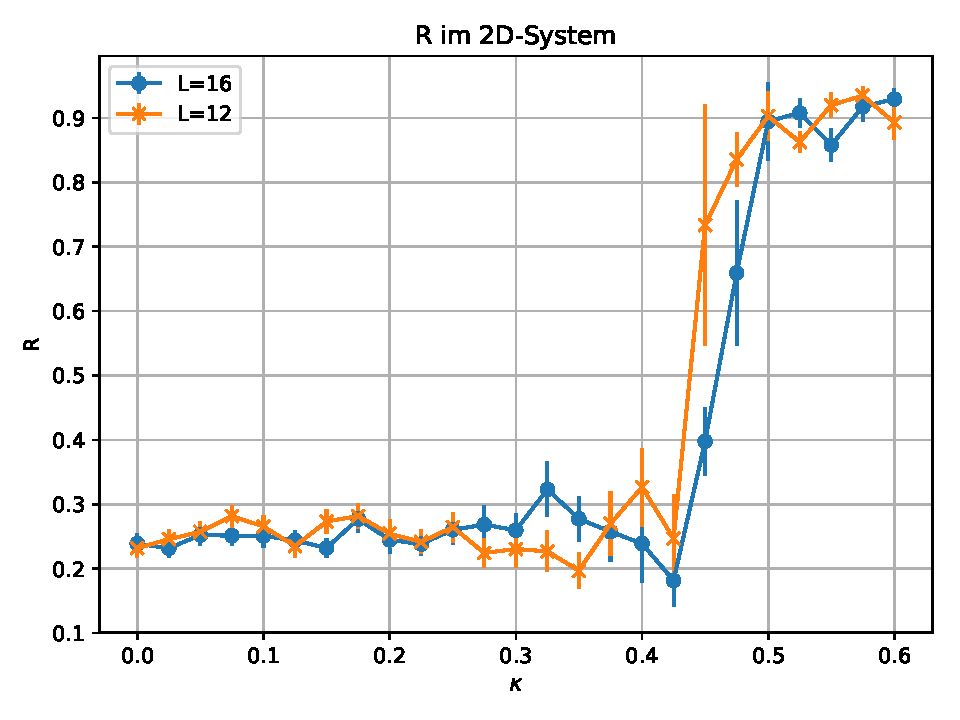
\includegraphics[width=\textwidth]{../figures/2dR.pdf}
  \caption{Bestimmung von $\kappa_c$ in 2 Dimensionen für verschiedene Systemgrößen $L$}\label{fig:2d}
\end{figure}

\begin{figure}
  \centering
  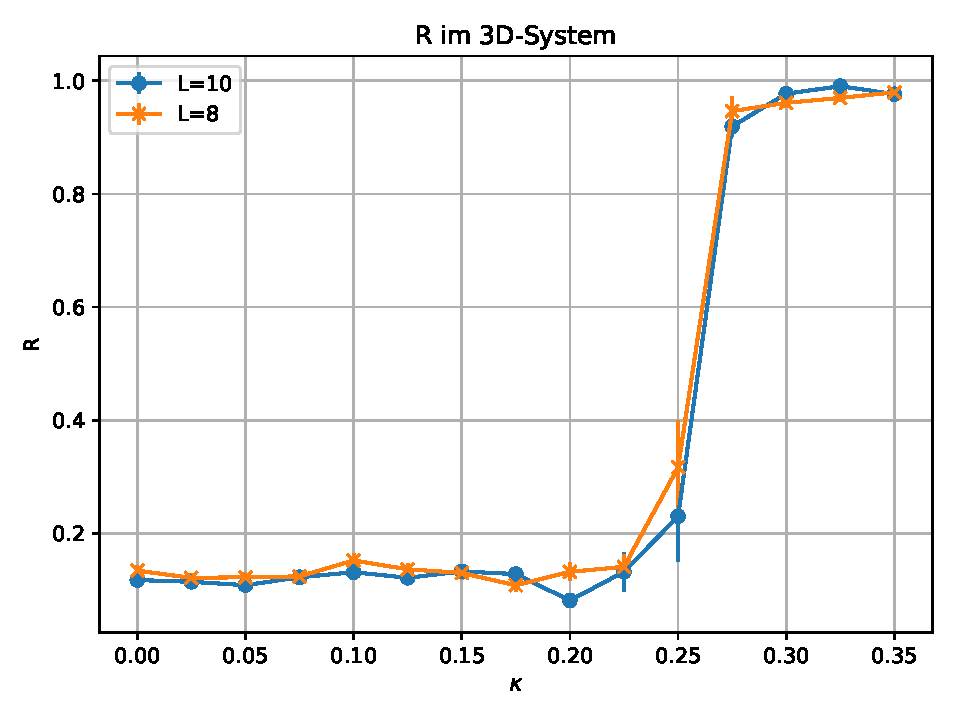
\includegraphics[width=\textwidth]{../figures/3dR.pdf}
  \caption{Bestimmung von $\kappa_c$ in 3 Dimensionen für verschiedene Systemgrößen $L$}\label{fig:3d}
\end{figure}

\begin{figure}
  \centering
  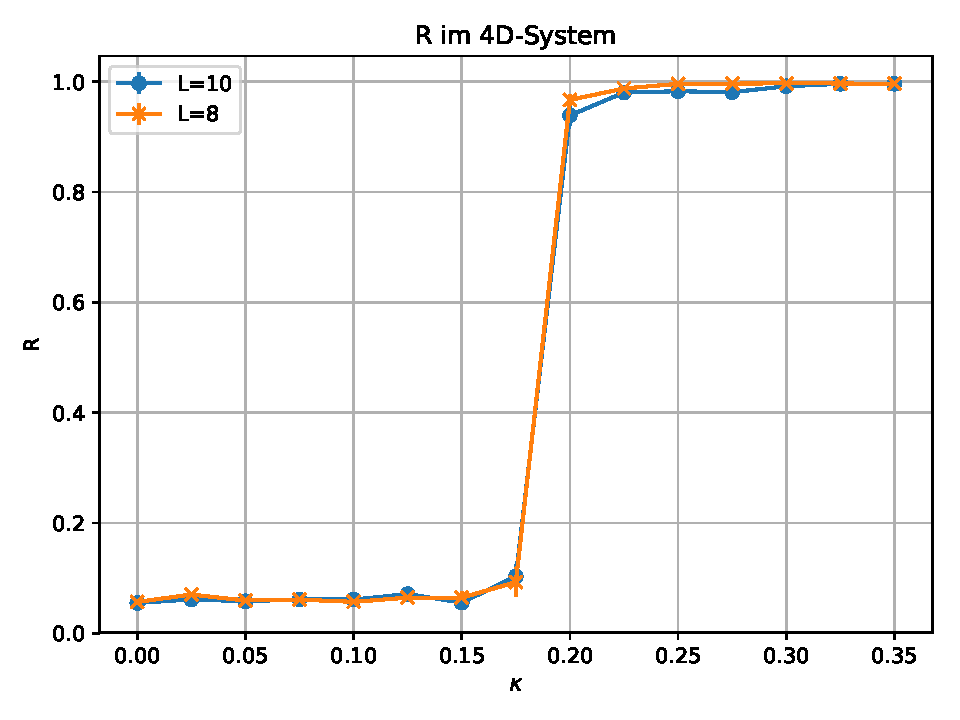
\includegraphics[width=\textwidth]{../figures/4dR.pdf}
  \caption{Bestimmung von $\kappa_c$ in 4 Dimensionen für verschiedene Systemgrößen $L$}\label{fig:4d}
\end{figure}

\section{Konvergenzverhalten von $R(\infty)$}

\subsection{Kosterlitz-Thouless-Phase}
Im XY-Modell wird für $R(L)$ in 2 Dimensionen in der Kosterlitz-Thouless-Phase
und große Systeme folgendes Konvergenzverhalten erwartet:
$R= 2^{-\frac{1}{4\pi \kappa}}$

Für verschiedene Systemgrößen und für $\kappa=0.5>\kappa_c$ wurde die Magnetisierung
gemessen und $R$ berechnet und graphisch dargestellt, siehe Abb.

\end{document}
